\section{Introduction}

In this chapter, we introduce the vision of what constitutes a Cognitive and
Immersive System, followed with a real-world implementation of various
components. As discussed in Chapter~\ref{chap:introduction}, we expect that
while a CAIS may be deployed into a variety of environments of differing
capabilities, they will all follow the same overarching definition and function.
For any given system, it is composed of three areas, that operate in a
cyclical flow, where sensors feed decision processes that feed output mechanisms.
However, at the core of this is that these systems are not just merely ``intelligent''
like prior art, where the room is able to answer queries about some problem domain,
but rather that it is ``cognitively intelligent'', where the system can reason
and answer questions about the cognitive states of agents and their cognitive
states towards the domain.

%%%%%%%%%%%%%%%%%%%%%%%%%%%%%%%%%%%%%%%%%%%%%%%%%%%%%%%%%%%%%%%%%%%%%%
\begin{figure}
    \centering
    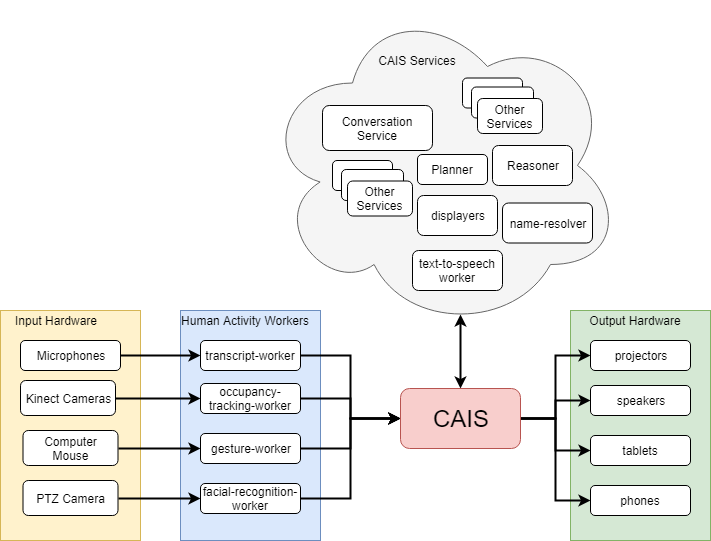
\includegraphics[width=0.5\columnwidth]{chapters/02_technology/figures/cais_high_level.png}
    \caption{High level diagram of CAIS architecture.}
    \label{fig:cycle-cais}
\end{figure}
%%%%%%%%%%%%%%%%%%%%%%%%%%%%%%%%%%%%%%%%%%%%%%%%%%%%%%%%%%%%%%%%%%%%%%

The requirements in question are cognitive in nature and exceed
intelligent rooms with sensors that can answer queries over simple
extensional data (e.g.\ a room that can answer financial queries such
as \textit{``Show me the number of companies with revenue over X?''}).
At a high-level, we require two conditions below hold:

\begin{itemize}
    \item $\mathcal{C}$ \emph{Cognitive}: A CAIS should be able to
      help agents with cognitive tasks and goals.  For instance, a
      system that simply aids in querying a domain $D$ is not
      cognitive in nature; a system that aids an agent in convincing
      another agent that some state-of-affairs holds in $D$ is
      considered cognitive. (Please see the appendix for more
      discussion of our usage of the term ``cognitive.'')
    \item $\mathcal{I}$ \emph{Immersive}:  There should
      be some attribute or property of a CAIS that is non-localized
      and distinguished from agents in the room.  Moreover, this
      property should be \textbf{common knowledge}.  (Note: this is
      not easily achievable with a physical robot, and this condition
      differentiates a CAIS from a cognitive
      agent.)\footnote{This condition may not strictly be realizable,
        but the goal is to at a minimum build systems that approach
        this ideal condition.}
\end{itemize}
